\section{Theoretischer Hintergrund}
\subsection{Elektrische Ladung}
Es gibt zwei verschiedene Arten von \textbf{Ladungen}, positive und negative Ladungen. Geladene Teilchen mit verschiedenen Vorzeichen ziehen sich an, Ladungen mit gleichem Vorzeichen stossen sich ab. \textbf{Elektrische Leiter} sind Materialien wie Metallen mit der Fähigkeit Ladungsträger zu transportieren. 
\begin{figure}[H]
\centering
\frame{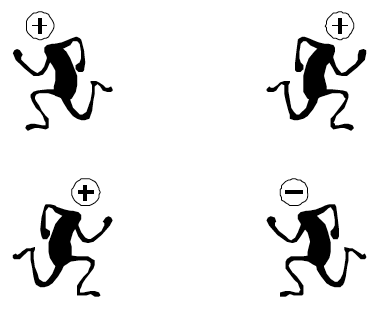
\includegraphics[scale=0.45]{../img/I/Ia}}
\caption{Gleiche Ladungen stossen sich ab, ungleiche ziehen sich an.}
\end{figure}
\subsection{Elektrischer Strom}
Die Ladungsmenge die während einer bestimmten Zeit durch den Leiter fliesst, ist ein Mass für die \textbf{Stromstärke}. Pro Sekunde fliessen $6.25\cdot 10^{18}$ Elektronen durch einen Draht. Die Einheit des elektrischen Stromes ist der \textbf{Ampére} $\text{A}$. Die Stromstärke ist das Verhältnis der transportierte Ladung $\triangle Q$ durch die Zeit $\triangle t$.
\begin{equation} 
\boxed{I=\dfrac{\triangle Q}{\triangle t},\quad [I]=\text{A}}
\end{equation} 
Messgeräte, mit denen der elektrische Storm gemessen wird, bezeichnet man als \textbf{Ampéremeter}. Um den in einem Leiter fliessenden elekltrischen Strom zu messen, muss dieser Leiter aufgetrennt und ein Ampéremeter eingeführt werden. 
\begin{figure}[H]
\centering
\frame{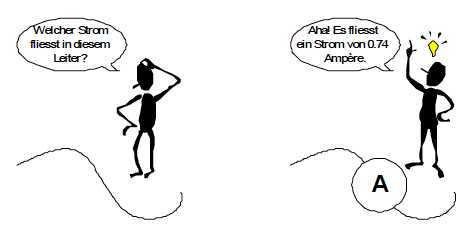
\includegraphics[scale=0.6]{../img/I/Ib}}
\caption{Der elektrische Strom wird duch Einschlaufen eines Ampèremeters in den Leiter gemessen.}
\end{figure}
Damit das Verhalten der Schaltung trotzdem möglichst nicht verändert wird, verhält sich ein gutes Ampèremeter wie ein Stück Leiter, das heisst wie ein \textbf{Kurzschluss}. 
\subsection{Elektrische Spannung}
Um eine Ladung zu bewegen muss \textbf{Arbeit} geleistet werden. Diese Arbeit ist umso grösser, je grösser die elektrische Spannung zwischen zwei benachbarten Punkten ist. Die Einheit der elektrischen Spannung ist das \textbf{Volt} $\text{V}$. Spannungen werden durch ein \textbf{Voltmeter} gemessen. Die Spannung wird immer zwischen zwei Punkten einer Schaltung gemessen.
\begin{figure}[H]
\centering
\frame{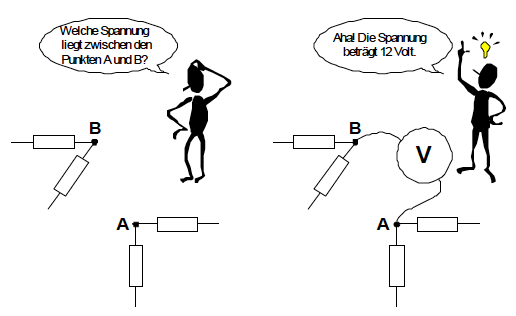
\includegraphics[scale=0.65]{../img/I/Ic}}
\caption{Die elektrische Spannung zwischen zwei Punkten wird mit einem Voltmeter gemessen.}
\end{figure}
Spannungen können auch durch einen Bezugspunkt oder \textbf{Massenpunkt} gemessen werden. Man spricht von der Spannung eines einzelnen Punktes und meint damit die Spannung zwischen dem Punkt und der Masse.
\subsection{Spannung-Strom-Kennlinie des Netzgeräts} 
Das Netzgerät liefert eine konstante Ausgangsspannung $U_{\text{konst}}$, solange der maximale Strom $I_{\text{max}}$ nicht überschritten wird. Versucht die angeschlossene Schaltung mehr Strom zu ziehen, schaltet das Netzgerät auf Konstantstrombetrieb um. Der Ausgangsstrom wird auf $I_{\text{max}}$ begrenzt. 
\begin{figure}[H]
\centering
\frame{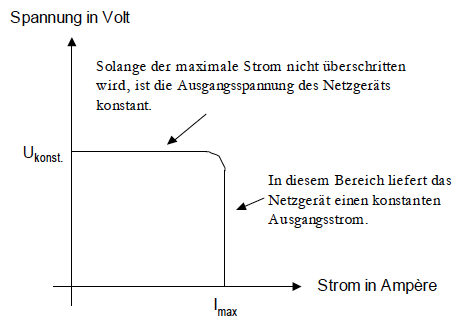
\includegraphics[scale=0.65]{../img/I/Id}}
\caption{Strom-Spannungs-Kennlinie des Netzgeräts}
\end{figure}
\subsection{Spannung-Strom-Kennlinie von Widerständen}
Die Spannung-Strom-Kennlinie eines Widerstands ist eine \textbf{Gerade}, die durch den Nullpunkt geht. Bei Verdoppelung der Spannung wird sich auch der Strom verdoppeln. Das Verhältnis von Spannung und Strom bleibt konstant und ist direkt proportional. Dadurch entsteht das \textbf{Ohmsche Gesetz}
\begin{equation}
\boxed{R=\dfrac{U}{I},\quad [R]=\Omega}
\end{equation}
\begin{figure}[H]
\centering
\frame{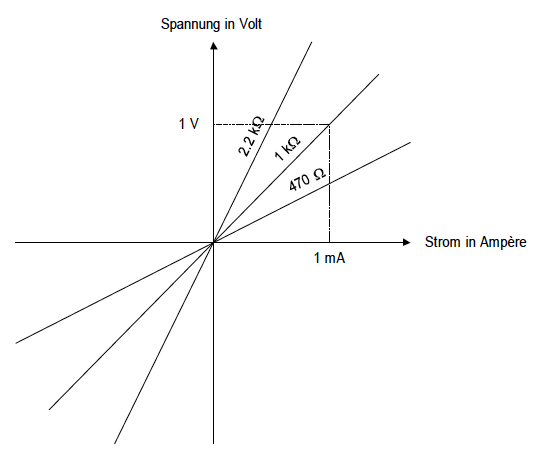
\includegraphics[scale=0.6]{../img/I/Ie}}
\caption{Strom-Spannungs-Kennlinie der drei Widerstände}
\end{figure}
\subsection{Spannung-Strom-Kennlinie der Glühlampe}
Die Spannung-Strom-Kennlinie einer Glühlampe ist keine Gerade. Das Verhältnis von Spannung zu Strom ist nicht konstant, sondern nimmt mit wachsender Spannung zu. Ist die Spannung klein, so leuchtet die Glühlampe schwach. Der Glühdraht ist relativ kalt und leitet den Strom besser. Der Widerstand des Drahtes steigt mit zunehmender Temperatur an. Die Glühlampe ist kein linearer ohmscher Widerstand. Das \textbf{Ohmsche Gesetz} gilt bedingt.
\begin{figure}[H]
\centering
\frame{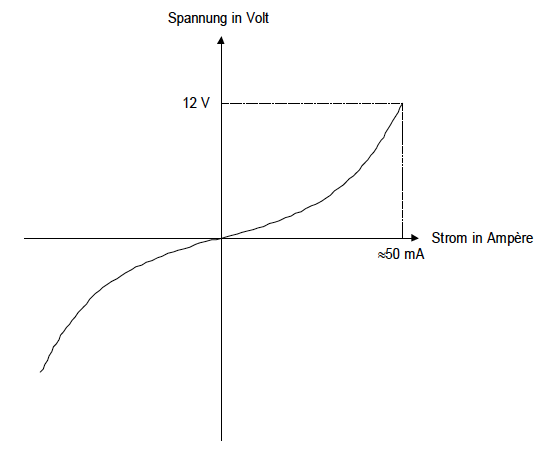
\includegraphics[scale=0.7]{../img/I/If}}
\caption{Strom-Spannungs-Kennlinie einer Glühlampe}
\end{figure} 
\subsection{Spannungsteiler}
Die Schaltung in Aufgabe 7 wird als Spannungsteiler bezeichnet. Die Eingangsspannung $U_{q}$ des Netzgeräts von 10 Volt wird in zwei Spannungen über den beiden Widerständen $R_1$ und $R_2$ aufgeteilt. 
\begin{figure}[H]
\centering
\frame{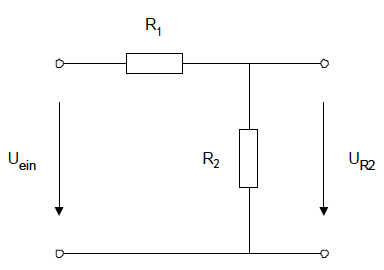
\includegraphics[scale=0.7]{../img/I/Ig}}
\caption{Spannungsteiler mit ohmschen Widerständen}
\end{figure} 
Durch beide Widerstände fliesst den gleichen Strom. Pro Sekunde fliessen eine gewissen Anzahl Elektronen durch $R_1$ und so fliessen gleiche Anzahl Elektronen durch $R_2$ pro Sekunde. Es gilt das \textbf{Ohmsche Gesetz} für beide Widerstände 
\begin{equation*}
\boxed{U_{R_1}=I\cdot R_{1}} \quad \boxed{U_{R_2}=I\cdot R_{2}}
\end{equation*}
Die \textbf{Summe} beider Spannungen beider Widerstände muss gleich der EIngangsspannung $U_Q$ sein. 
\begin{equation*}
U_{q}=U_{R_1}+U_{R_2}=I\cdot R_1+I\cdot R_2=I\cdot \left(R_1+R_2\right)
\end{equation*}
Somit fliesst ein Strom von
\begin{equation*}
I=\dfrac{U_Q}{R_1+R_2}
\end{equation*}
Die Spannungen an den jeweiligen Widerständen lauten
\begin{equation}
\boxed{U_{R_1}=\dfrac{U_Q}{R_1+R_2}\cdot R_1}\quad \boxed{U_{R_2}=\dfrac{U_Q}{R_1+R_2}\cdot R_2}
\end{equation}
\section{Versuchsanleitung}
\subsection{Messgeräte}
Für diesen Versuch wurden ein \textbf{Labornetzgerät} und zwei Multimeter benötigt. Ein Labornetzgerät liefert eine \textbf{konstante, einstellbare Spannung}. Die elektrische Spannung zwischen den beiden Anschlüssen des Netzgeräts ist, unabhängig von der Belastung, immer gleich.
\begin{figure}[H]
\centering
\frame{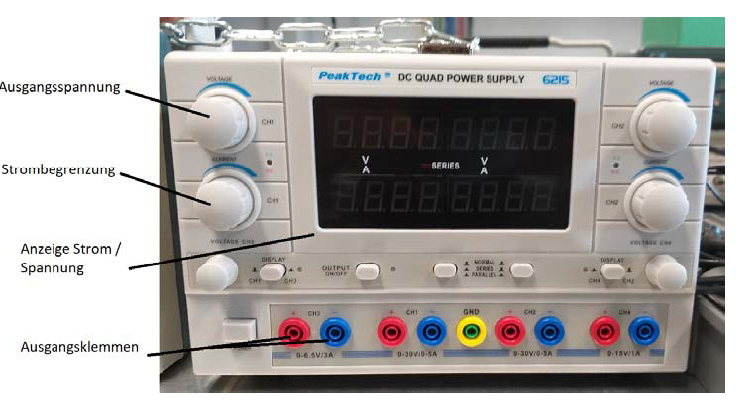
\includegraphics[scale=0.7]{../img/I/Ih}}
\caption{Frontplatte des Labornetzgeräts}
\end{figure} 
Um das Netzgerät und/oder die angeschlossene Schaltung zu schützen kann jedoch der \textbf{maximale Ausgangsstrom} begrenzt werden. Zieht die angeschlossene Schaltung einen höheren Strom, so wird die Ausgangsspannung solange verkleinert, bis der Strom wieder im erlaubten Bereich liegt.
\\\\
Wird das Netzgerät als Konstantspannungsquelle gebraucht, so muss man darauf achten, dass die Strombegrenzung nicht anspricht.
\begin{figure}[H]
\centering
\frame{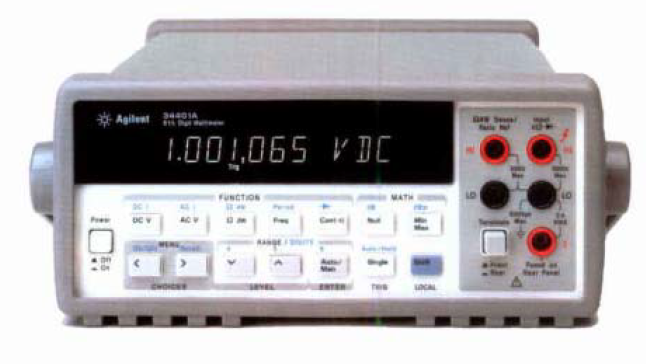
\includegraphics[scale=0.7]{../img/I/Ii}}
\caption{Frontplatte des Multimeters}
\end{figure} 
Anstelle der Volt- und Ampéremeter werden \textbf{Multimeter} benutzt. Die Umschaltung erfolgt über einen Wahlschalter oder über Funktionstasten. Da sich ein Ampéremeter wie ein Kurzschluss verhält, ist es nicht ratsam, damit Spannung messen zu wollen. Moderne Multimeter können neben Spannung und Strom auch andere Grössen wie beispielsweise Widerstand, Kapazität, Frequenz und Stromverstärkung messen.
\subsection{Widerstände}
Ein \textbf{Widerstand} wird durch sein Widerstandswert beschrieben. Die Einheit des Widerstandes ist das Ohm ($\Omega$). Häufig werden Widerstände deshalb mit Farbringen gekennzeichnet. Die ersten zwei (manchmal drei) Ringe geben die ersten zwei (resp. drei) Ziffern des Widerstandswerts an. Der nachfolgende Ring gibt einen Multiplikator an, mit dem die Ziffern multipliziert werden. Der letzte Ring bezeichnet die Toleranz des Widerstands. 
\begin{figure}[H]
\centering
\frame{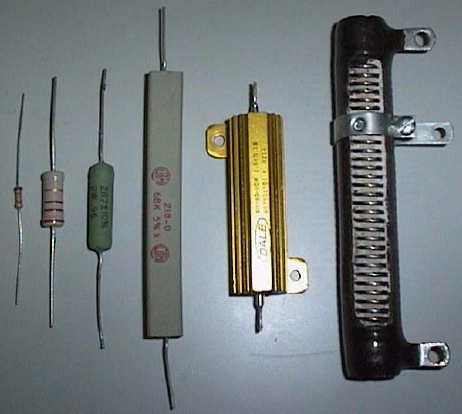
\includegraphics[scale=0.6]{../img/I/Ij}}
\caption{Verschiedene Bauformen von Widerständen}
\end{figure} 
\begin{figure}[H]
\centering
\frame{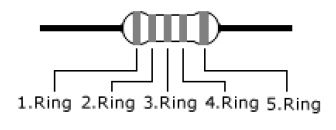
\includegraphics[scale=0.7]{../img/I/Ik}}
\caption{Kennzeichnung des Widerstandswerts.}
\end{figure} 
\begin{table}[H]
\centering
\begin{tabular}{cccccc}\hline
Farbe &1. Ring &2.Ring &3.Ring &4. Ring &5. Ring\\\hline
Silber&•& •& •&x0,01& $\pm$10\%\\
Gold&•& •& •& x0,1& $\pm$5\%\\
Schwarz&•& 0& 0&x1 &•\\
Braun&1& 1& 1&x10& $\pm$1\%\\
Rot&2 &2 &2& x100& $\pm$2\%\\
Orange&3 &3& 3&x1000& •\\
Gelb&4 &4 &4& x10000& •\\
Gruen&5 &5& 5&x100000&$\pm$ 0.5\%\\
Blau&6 &6 &6&x1000000&$\pm$0.25\%\\
Lila&7 &7& 7&x10000000&$\pm$0.1\%\\
Grau&8 &8& 8&•&$\pm$0.05\%\\
Weiss& 9& 9& 9& •& •\\\hline
\end{tabular}
\caption{Widerstandwerte mittels Farbringen.}
\end{table}
\subsection{Aufgaben}
\subsubsection{Aufgabe 1}
Stellen Sie die Spannung am Netzgerät auf das \textbf{Minimum} und drehen Sie die Strombegrenzung auf \textbf{``max''}. Wählen Sie beim Multimeter die Funktion \textbf{``DC V''} (Messen von Gleichspannung) und schliessen Sie das Multimeter an die Ausgangsklemmen des Netzgeräts an. 
\begin{enumerate}[$a)$]
\item In welchem Bereich können Sie die Ausgangsspannung des Netzgeräts einstellen? 
\item Wie genau ist die Anzeige der Ausgangsspannung des Netzgeräts in \% beim \textbf{Maximum} bez. Multimeter?
\end{enumerate}
\subsubsection{Aufgabe 2}
Stellen Sie die Spannung am Netzgerät auf ca. $10\text{V}$ und drehen Sie nun die Strombegrenzung auf \textbf{``min''} (nur soweit, dass noch die Ausgangsspannung anliegt). Schliessen Sie das Multimeter an die Ausgangsklemmen des Netzgeräts an. Wählen Sie wiederum die Funktion \textbf{``DC I''} (Messen von Gleichstrom).
\begin{enumerate}[$a)$]
\item In welchem Bereich können Sie den Ausgangsstrom des Netzgeräts einstellen? Welchen maximalen Strom kann das Netzgerät liefern? 
\item Welchen Wert zeigt das Voltmeter am Netzgerät an?
\end{enumerate}
\subsubsection{Aufgabe 3}
Bauen Sie die unten stehende Messschaltung auf. Achten Sie darauf, beim als Ampèremeter benutzten Multimeter den Eingang für hohe Ströme zu verwenden. Drehen Sie den Knopf für die Strombegrenzung auf \textbf{``max''} und wählen Sie eine \textbf{mittlere Ausgangsspannung}.
\begin{figure}[H]
\centering
\frame{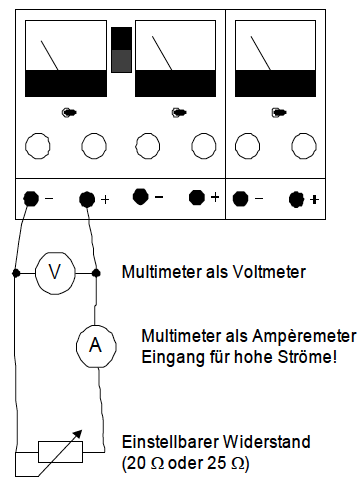
\includegraphics[scale=0.7]{../img/I/Il}}
\caption{Aufbau Aufgabe 3}
\end{figure} 
\begin{enumerate}[$a)$]
\item Verändern Sie nun den Wert des einstellbaren Widerstands und tragen Sie die jeweils gemessenen Spannungs- und Stromwerte in eine Tabelle ein.
\begin{table}[H]
\centering
\begin{tabular}{ccc}\hline
$U/\text{V}$&$I/\text{A}$&$R/\Omega$\\\hline
&&\\
&&\\
&&\\
&&\\
&&\\\hline
\end{tabular}
\caption{Spannungs- und Stromwerte von $20\Omega$}
\end{table}
\item Stellen Sie die Werte der Tabelle graphisch dar (separates Blatt), indem Sie diese in ein Koordinatensystem eintragen. Diese Kurve nennt man die Spannung-Strom-Kennlinie des Netzgeräts, da sie den Zusammenhang zwischen Strom und Spannung wiedergibt. 
\begin{figure}[H]
\centering
\frame{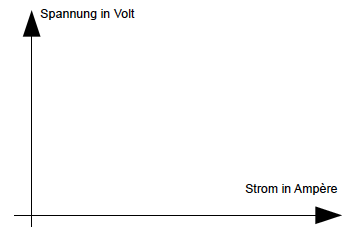
\includegraphics[scale=0.7]{../img/I/Im}}
\caption{Spannungs-Strom-Kennlinie von $20\Omega$}
\end{figure}
\item Kommentieren Sie die erhaltene Kennlinie.
\end{enumerate}
\subsubsection{Aufgabe 4}
Wechseln Sie nun den einstellbaren Widerstand in der obigen Schaltung durch einen fixen Widerstand von $1000\Omega$ (1$\text{k}\Omega$) aus. Drehen Sie die Strombegrenzung auf \textbf{``max''}.
\begin{enumerate}[$a)$]
\item Ändern Sie die Ausgangsspannung des Netzgeräts und tragen Sie die jeweils gemessenen Spannungs- und Stromwerte in eine Tabelle ein. 
\begin{table}[H]
\centering
\begin{tabular}{ccc}\hline
$U/\text{V}$&$I/\text{A}$&$R/\Omega$\\\hline
&&\\
&&\\
&&\\
&&\\
&&\\\hline
\end{tabular}
\caption{Spannungs- und Stromwerte von $1\text{k}\Omega$}
\end{table}
\item Um auch negative Spannungs- und Stromwerte zu erhalten, müssen Sie die Anschlüsse am Netzgerät vertauschen. 
\item Stellen Sie diese Werte in einer Spannung-Strom-Kennlinie graphisch dar. 
\begin{figure}[H]
\centering
\frame{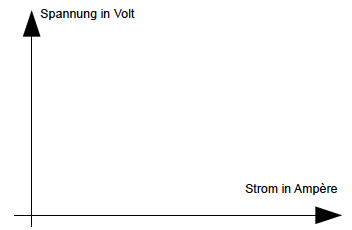
\includegraphics[scale=0.7]{../img/I/Imm}}
\caption{Spannungs-Strom-Kennlinie von $1\text{k}\Omega$}
\end{figure}
\item Welche Kurvenform erhalten Sie? 
\item Tragen Sie in die Tabelle auch den Wert ``Spannung dividiert durch Strom'' ein.
\end{enumerate}
\subsubsection{Aufgabe 5}
Wiederholen Sie die \textbf{Aufgabe 4} mit Widerständen von 470$\Omega$ und 2.2$\text{k}\Omega$.
\begin{table}[H]
\centering
\begin{tabular}{ccc}\hline
$U/\text{V}$&$I/\text{A}$&$R/\Omega$\\\hline
&&\\
&&\\
&&\\
&&\\
&&\\\hline
\end{tabular}
\caption{Spannungs- und Stromwerte von $470\Omega$}
\end{table} 
\begin{table}[H]
\centering
\begin{tabular}{ccc}\hline
$U/\text{V}$&$I/\text{A}$&$R/\Omega$\\\hline
&&\\
&&\\
&&\\
&&\\
&&\\\hline
\end{tabular}
\caption{Spannungs- und Stromwerte von $2.2\text{k}\Omega$}
\end{table} 
\begin{enumerate}[$a)$]
\item Zeichnen Sie die Strom-Spannungs-Kennlinie für alle drei Widerstände in einem gemeinsamen Koordinatensystem ein. 
\begin{figure}[H]
\centering
\frame{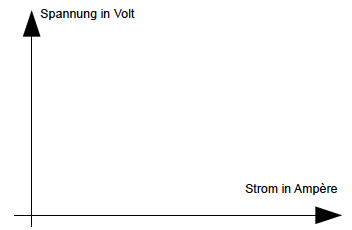
\includegraphics[scale=0.7]{../img/I/Immm}}
\caption{Spannungs-Strom-Kennline von $470\Omega$ und $1\text{k}\Omega$}table
\end{figure}
\item Was können Sie über die Steigungen der Geraden aussagen?
\end{enumerate}
\subsubsection{Aufgabe 6}
Wiederholen Sie die \textbf{Aufgabe 4}, indem Sie den Widerstand durch eine \textbf{Glühlampe} ersetzen. Achten Sie darauf, dass die Spannung nun $12\text{V}$ nicht mehr überschreiten darf!
\begin{enumerate}[$a)$] 
\item Zeichnen Sie wiederum die Spannung-Strom-Kennlinie der Glühlampe auf. 
\begin{table}[H]
\centering
\begin{tabular}{ccc}\hline
$U/\text{V}$&$I/\text{A}$&$R/\Omega$\\\hline
&&\\
&&\\
&&\\
&&\\
&&\\\hline
\end{tabular}
\caption{Spannungs- und Stromwerte der Glühlampe}
\end{table}
\item Vergleichen Sie diese mit den Kennlinien der vorhergehenden Versuche.
\begin{figure}[H]
\centering
\frame{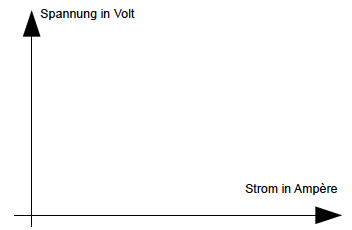
\includegraphics[scale=0.7]{../img/I/Immmm}}
\caption{Spannungs-Strom-Kennlinie der Glühlampe}
\end{figure}
\end{enumerate}
\subsubsection{Aufgabe 7}
\begin{figure}[H]
\centering
\frame{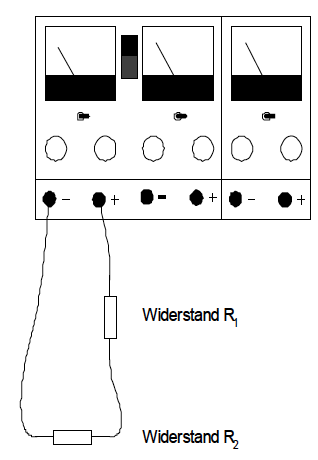
\includegraphics[scale=0.7]{../img/I/In}}
\caption{Spannungsteiler}
\end{figure} 
Bauen Sie die nebenstehende Versuchsanordnung auf. Wählen Sie eine Ausgangsspannung des Netzgeräts von genau $10\text{V}$. Füllen Sie nun die unten stehende Tabelle aus.
\begin{table}[H]
\centering
\begin{tabular}{cccc}\hline
$R_1/\Omega$&$R_2/\Omega$&$U_{R_1}/\text{V}$&$U_{R_2}/\text{V}$\\\hline
$1000$&$1000$&\\
$1000$&$470$&\\
$2200$&$1000$&\\
$1000$&$0$&\\
$0$&$1000$&\\\hline
\end{tabular}
\caption{Spannungen über die Widerstände}
\end{table}
\begin{enumerate}[$a)$]
\item Was können Sie über die Summe der beiden Spannungen aussagen?
\item Versuchen Sie eine Beziehung herzuleiten, mit der sie die Spannung über $R_2$ als Funktion der beiden Widerstandswerte $R_1$ und $R_2$ berechnen können.
\begin{equation*}
\boxed{U_{R_1}=I\cdot R_{1}} \quad \boxed{U_{R_2}=I\cdot R_{2}}
\end{equation*}
Die \textbf{Summe} beider Spannungen beider Widerstände muss gleich der EIngangsspannung $U_Q$ sein. 
\begin{equation*}
U_{q}=U_{R_1}+U_{R_2}=I\cdot R_1+I\cdot R_2=I\cdot \left(R_1+R_2\right)
\end{equation*}
Somit fliesst ein Strom von
\begin{equation*}
I=\dfrac{U_Q}{R_1+R_2}
\end{equation*}
Die Spannungen an den jeweiligen Widerständen lauten
\begin{equation}
\boxed{U_{R_1}=\dfrac{U_Q}{R_1+R_2}\cdot R_1}\quad \boxed{U_{R_2}=\dfrac{U_Q}{R_1+R_2}\cdot R_2}
\end{equation}
\end{enumerate}
\section{Diskussion}